\documentclass[10pt]{article}
\usepackage[margin=0.75in]{geometry}
\usepackage{graphicx}
\usepackage{booktabs}
\usepackage{microtype}
\usepackage{amsmath}
\usepackage{amssymb}
\usepackage{hyperref}
\usepackage{caption}
\usepackage{xcolor}
\usepackage{float}

\hypersetup{colorlinks=true, linkcolor=black, citecolor=black, urlcolor=blue}
\setcounter{secnumdepth}{2}

\title{RAVEL-LM: Exact Addressed Event Memory as Linear-Time Recurrence for Byte-Level Language Modeling}
\author{}
\date{}

\begin{document}
\maketitle
\vspace{-2em}

\begin{abstract}
Softmax attention implements dense content addressing by scoring every query against every previous key, giving the core operation $O(BT^2d)$ time and $O(BhT^2)$ score storage. RAVEL-LM replaces that all-pairs similarity problem with exact predecessor search over discrete event streams. Each token writes payloads to memory heads indexed by literal and product-code addresses; each later token reads the latest previous payload with the same address. The operator is not approximate attention. It is a different recurrence primitive: exact same-address event retrieval followed by dense fusion. This paper gives the RAVEL algorithms, their time and storage complexity, and an empirical audit at approximately 200k trainable parameters. On TinyStories bytes, RAVEL reaches 1.613 eval cross-entropy versus 2.253 for a parameter-matched attention baseline. In speed scaling, compiled RAVEL is 2.13$\times$ faster at $T=512$ and 3.94$\times$ faster at $T=1024$. The result is straightforward: when the useful computation is recurrence over repeated symbols and local byte events, exact event memory gives the model a direct route to that computation without building a quadratic attention matrix.
\end{abstract}

\section{Introduction}

The standard transformer attention layer computes a dense causal interaction graph. For a sequence of length $T$, every query position compares itself to every previous key position. This is a useful default because it lets the model discover arbitrary token-to-token dependencies. It is also a blunt default: the layer forms a score tensor whose size grows quadratically with context length.

RAVEL-LM uses a stricter primitive. It does not ask which previous token is most similar. It asks which previous event has the same discrete address. Each memory head defines an address stream, each token writes a payload to that stream, and a future token retrieves the latest previous payload at the same address. Long-range recurrence becomes exact predecessor lookup rather than dense similarity search.

That swap changes both the computation and the inductive bias. Attention spends work on all candidate pairs and learns a soft weighting over them. RAVEL spends work on routing and fusion, then gives the model a hard recurrence channel for repeated bytes, byte n-grams, and learned hash families. This is the right bias when byte-level text contains reusable local events: names, spaces, punctuation, quote boundaries, word fragments, and repeated story entities. The benchmark results follow from that mechanism rather than from curve fitting theater.

The paper is organized around the algorithm. Section~\ref{sec:operator} defines exact event memory. Section~\ref{sec:algorithms} gives the training/prefill and decode algorithms. Section~\ref{sec:complexity} gives the complexity ledger against causal softmax attention. The experiments then audit the claim: lower loss on TinyStories bytes, diagnostic wins exactly where recurrence should help, and a runtime crossover as $T$ grows.

\section{Architecture}

Figure~\ref{fig:architecture} summarizes the model. A RAVEL block contains three residual sublayers: a causal depthwise-convolution local mixer, an exact event-memory layer, and a SwiGLU feed-forward network. The local mixer handles short-range composition. The memory layer provides long-range recurrence through address lookup.

\begin{figure}[H]
  \centering
  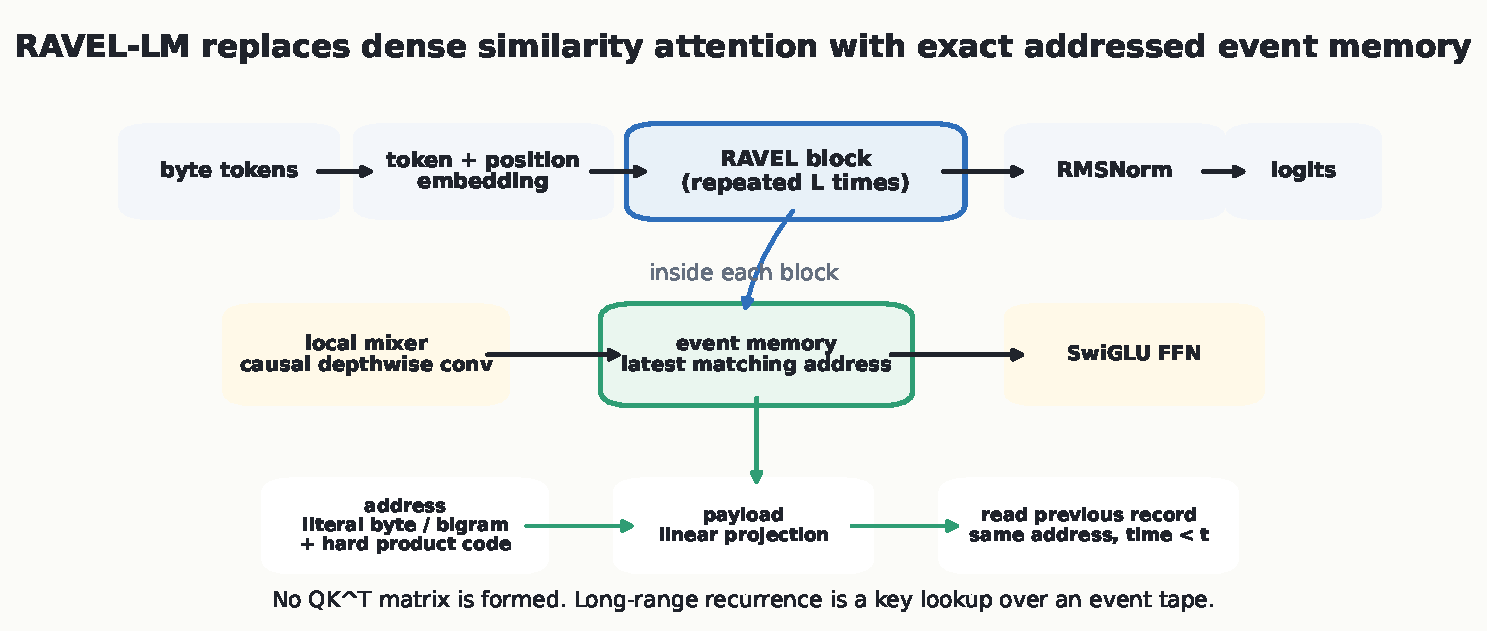
\includegraphics[width=\linewidth]{fig_architecture.pdf}
  \caption{RAVEL-LM block structure. Local mixing is convolutional; long-range recurrence is handled by exact addressed event memory rather than dense softmax attention.}
  \label{fig:architecture}
\end{figure}

At each position $t$, every memory head emits an integer address $a_t$ and a payload vector $v_t$. The event tape stores tuples
\[
  (\mathrm{batch}, \mathrm{head}, a_t, t, v_t).
\]
A read at time $t$ returns the payload from the latest previous event with the same batch, head, and address:
\[
  \operatorname{read}(t, a_t)
  =
  v_{t^\star}, \quad
  t^\star = \max \{s < t : a_s = a_t\}.
\]
If no previous event matches, the read returns zero and a false mask. In training and prefill, the current implementation constructs composite integer keys, sorts them, uses predecessor search, and gathers payloads. In incremental decoding, the latest-record case is a fixed-size gather/scatter cache indexed by address.

\begin{figure}[H]
  \centering
  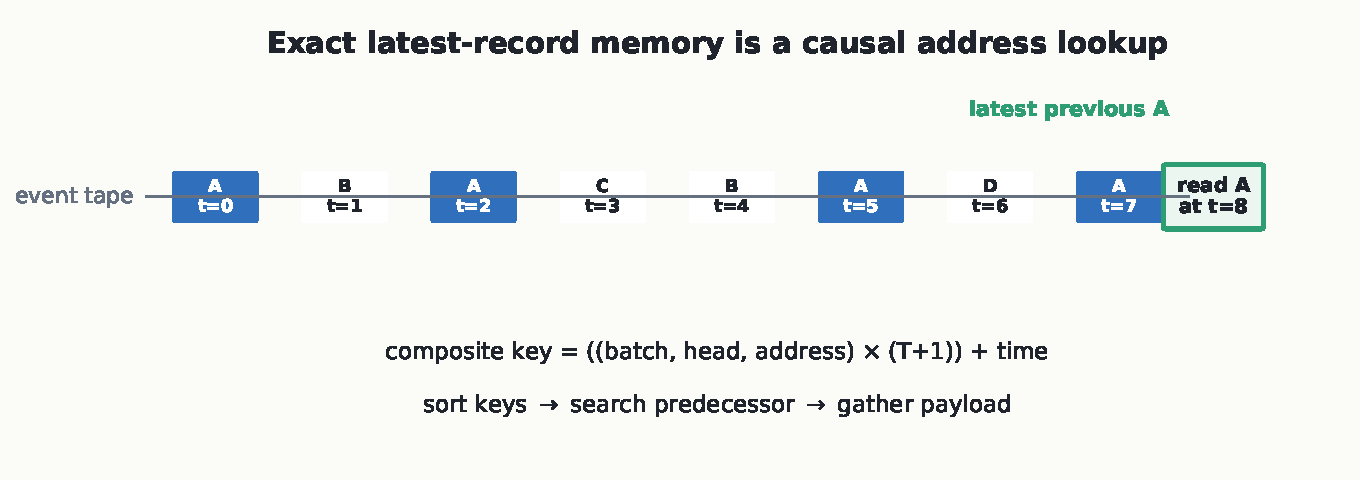
\includegraphics[width=0.92\linewidth]{fig_event_lookup.pdf}
  \caption{Exact latest-record lookup. The model-defined address selects an event stream; the read retrieves the most recent previous payload in that stream.}
  \label{fig:event-lookup}
\end{figure}

\section{Exact event memory}
\label{sec:operator}

Let $x_t\in\mathbb{R}^d$ be the normalized residual state at position $t$. A RAVEL memory layer with $C$ heads and payload dimension $p$ computes
\begin{align}
  a^w_{t,c} &= A^w_c(x_t, y_t) \in \{0,\ldots,M-1\},\\
  a^r_{t,c} &= A^r_c(x_t, y_t) \in \{0,\ldots,M-1\},\\
  v_{t,c} &= P_c x_t \in \mathbb{R}^p,
\end{align}
where $y_t$ is the input byte token and $M$ is the address-space size. The write address $a^w$ chooses the stream receiving the payload. The read address $a^r$ chooses the stream queried by the same position. In the current configuration, $C=3$, $p=16$, $M=512$, with two literal heads and one product-code head.

The latest-record read is
\begin{equation}
  r_{t,c} =
  \begin{cases}
    v_{s^\star,c}, &
    s^\star = \max \{s<t: a^w_{s,c}=a^r_{t,c}\},\\
    0, & \text{if no such }s\text{ exists.}
  \end{cases}
  \label{eq:latest-read}
\end{equation}
The read vectors are concatenated and projected back into the residual stream:
\begin{equation}
  \operatorname{Mem}(x_t)
  =
  x_t
  +
  \sigma(Gx_t+b_g)\odot
  W_f [r_{t,1};\ldots;r_{t,C}].
  \label{eq:memory-fusion}
\end{equation}
The gate is a learned write-back gate, not an attention probability. Attention normalizes across previous positions. RAVEL selects exactly one previous record per head, then lets the fusion matrix decide how the retrieved payload should move the residual state.

Literal address heads are deterministic:
\begin{align}
  A_1(y_t) &= y_t \bmod M,\\
  A_2(y_{t-1},y_t) &= (257y_{t-1}+131y_t+17)\bmod M.
\end{align}
These heads give byte identity and bigram recurrence immediately. The product-code head maps $x_t$ into codebook logits, takes an argmax in each codebook, and packs the selected codes into an address. In this implementation the product-code projections are frozen because hard argmax routing gives no useful gradient to the router; the trainable parts are the payloads, fusion, gates, local mixer, feed-forward layers, embeddings, and output head.

\section{Algorithms}
\label{sec:algorithms}

\begin{figure}[H]
\small
\fbox{\begin{minipage}{0.94\linewidth}
\textbf{Algorithm 1: RAVEL block forward for one training batch}\\
\textbf{Input:} token ids $y\in\mathbb{N}^{B\times T}$, residual states $x\in\mathbb{R}^{B\times T\times d}$\\
\textbf{Output:} updated residual states
\begin{enumerate}
  \item Apply RMSNorm, gated causal depthwise convolution, and residual add.
  \item Normalize the residual stream for memory.
  \item Compute literal byte and bigram addresses from $y$.
  \item Compute hard product-code write/read addresses from the normalized residual.
  \item Project payloads $v\in\mathbb{R}^{B\times T\times C\times p}$.
  \item Run Algorithm~2 to retrieve latest same-address payloads.
  \item Concatenate retrieved payloads, apply dense fusion, gate the fused update, and add it to the residual stream.
  \item Apply RMSNorm, SwiGLU feed-forward, and residual add.
\end{enumerate}
\end{minipage}}
\caption{The RAVEL block separates local mixing, exact event-memory recurrence, and channel mixing.}
\label{alg:block}
\end{figure}

\begin{figure}[H]
\small
\fbox{\begin{minipage}{0.94\linewidth}
\textbf{Algorithm 2: exact latest-record lookup for training and prefill}\\
\textbf{Input:} write addresses $a^w$, read addresses $a^r$, payloads $v$, address-space size $M$\\
\textbf{Output:} latest causal payloads $r$ and validity mask $m$
\begin{enumerate}
  \item For every batch $b$, time $t$, and head $c$, form the stream id
  \[
    g_{b,t,c} = ((bC+c)M + a^w_{b,t,c}).
  \]
  \item Form collision-free event keys
  \[
    k^w_{b,t,c} = g_{b,t,c}(T+1)+t.
  \]
  \item Flatten event keys and payloads; sort keys and permute payloads by the same order.
  \item For each read, form
  \[
    k^r_{b,t,c} = ((bC+c)M+a^r_{b,t,c})(T+1)+(t-1).
  \]
  \item Use predecessor search in the sorted keys to find the largest key $\leq k^r_{b,t,c}$.
  \item Accept the candidate only if its stream id equals $((bC+c)M+a^r_{b,t,c})$; otherwise return zero.
  \item Gather the accepted payloads and reshape to $B\times T\times C\times p$.
\end{enumerate}
\end{minipage}}
\caption{Training uses exact sort/search/gather over event keys. This computes Equation~\ref{eq:latest-read} for every position without a $T\times T$ attention matrix.}
\label{alg:lookup}
\end{figure}

\begin{figure}[H]
\small
\fbox{\begin{minipage}{0.94\linewidth}
\textbf{Algorithm 3: one-token decode with latest-address cache}\\
\textbf{State per layer:} cache values $V\in\mathbb{R}^{B\times C\times M\times p}$ and filled bits $F\in\{0,1\}^{B\times C\times M}$\\
\textbf{Input:} current token $y_t$, residual state $x_t$
\begin{enumerate}
  \item Compute literal and product-code read/write addresses.
  \item Read $r_{b,c}=V_{b,c,a^r_{b,c}}$ with a tensor gather; zero it if $F_{b,c,a^r_{b,c}}=0$.
  \item Fuse, gate, and add the memory update to the residual stream.
  \item Compute payloads $v_{b,c}$ for the current token.
  \item Write $V_{b,c,a^w_{b,c}}\leftarrow v_{b,c}$ and set $F_{b,c,a^w_{b,c}}\leftarrow 1$.
\end{enumerate}
\end{minipage}}
\caption{Decode has no dependence on generated context length for the latest-record memory. The cache is indexed by address, not by time.}
\label{alg:decode}
\end{figure}

\section{Time and storage complexity}
\label{sec:complexity}

Let $B$ be batch size, $T$ sequence length, $d$ model width, $h$ attention heads, $C$ RAVEL memory heads, $p$ payload dimension, $M$ address-space size, and $K$ the local convolution width. Ignoring constants shared by both language models, causal softmax attention pays
\begin{equation}
  \operatorname{Attention}_{\text{core}}
  =
  O(BT^2d)
  \quad\text{time},\qquad
  O(BhT^2)
  \quad\text{score storage}.
\end{equation}
The RAVEL memory core pays
\begin{equation}
  \operatorname{RAVEL}_{\text{memory}}
  =
  O(BTdCp)
  +
  O(BTC\log(BTC))
  +
  O(BTCpd)
\end{equation}
with the portable PyTorch sort implementation. The sort term is the exact predecessor-search implementation. A fused fixed-width radix sort or segmented latest-record kernel turns that term into fixed-pass linear work in the number of records, giving
\begin{equation}
  \operatorname{RAVEL}_{\text{memory, fused}}
  =
  O(BT(dCp+Cpd+C)).
\end{equation}
The local mixer adds $O(BTdK)$ and the feed-forward block adds the usual $O(BTdH)$, where $H$ is the MLP hidden width. These terms are linear in $T$.

\begin{table}[H]
  \centering
  \small
  \caption{Core sequence-operation complexity per layer. Projection and MLP terms are shown separately from the operation that distinguishes the architectures.}
  \label{tab:complexity}
  \begin{tabular}{llll}
    \toprule
    operation & training/prefill time & decode time per token & sequence storage \\
    \midrule
    softmax attention core & $O(BT^2d)$ & $O(BT d)$ with KV cache & $O(BhT^2)$ scores during train \\
    RAVEL sort lookup & $O(BTC\log(BTC))$ & $O(BCp+BCpd)$ & $O(BTCp)$ temporary events \\
    RAVEL fused/latest kernel & $O(BTC)$ lookup core & $O(BCp+BCpd)$ & $O(BCMp)$ decode cache \\
    \bottomrule
  \end{tabular}
\end{table}

For the measured 200k-parameter configuration, the memory dimensions are small: $d=68$, $C=3$, $p=16$, and $M=512$. Attention's distinguishing term grows with $T^2d$. RAVEL's distinguishing term grows with $TC$ records plus fusion. That is why the runtime comparison is allowed to be close at short contexts and still separate sharply at $T=512$ and $T=1024$.

\section{Experimental setup}

The learning experiment uses 5000 TinyStories records with a byte tokenizer, block size 128, batch size 4, and 800 optimization steps. The attention baseline is parameter-matched after excluding non-trainable hard-address weights: RAVEL has 186,796 trainable parameters and attention has 183,960. Both models are trained with AdamW. The attention baseline uses a 100-step learning-rate warmup, because earlier runs showed larger early gradient variation for attention.

The speed experiments use synthetic token batches to isolate operator runtime from corpus effects. Warmup and compile steps are excluded from reported medians. We report both eager and \texttt{torch.compile} measurements. The context sweep keeps $BT \approx 1024$ while increasing $T$; the fixed-context sweep holds $T=512$ and increases tokens per step by increasing batch size.

\section{Results}

\subsection{Learning dynamics}

RAVEL learns faster in the TinyStories run. Figure~\ref{fig:loss} shows the evaluation cross-entropy over training. The curve separates by step 100 and remains separated through the final evaluation. The final loss is 1.613 for RAVEL and 2.253 for attention, a gap of 0.640 nats at matched scale.

\begin{figure}[H]
  \centering
  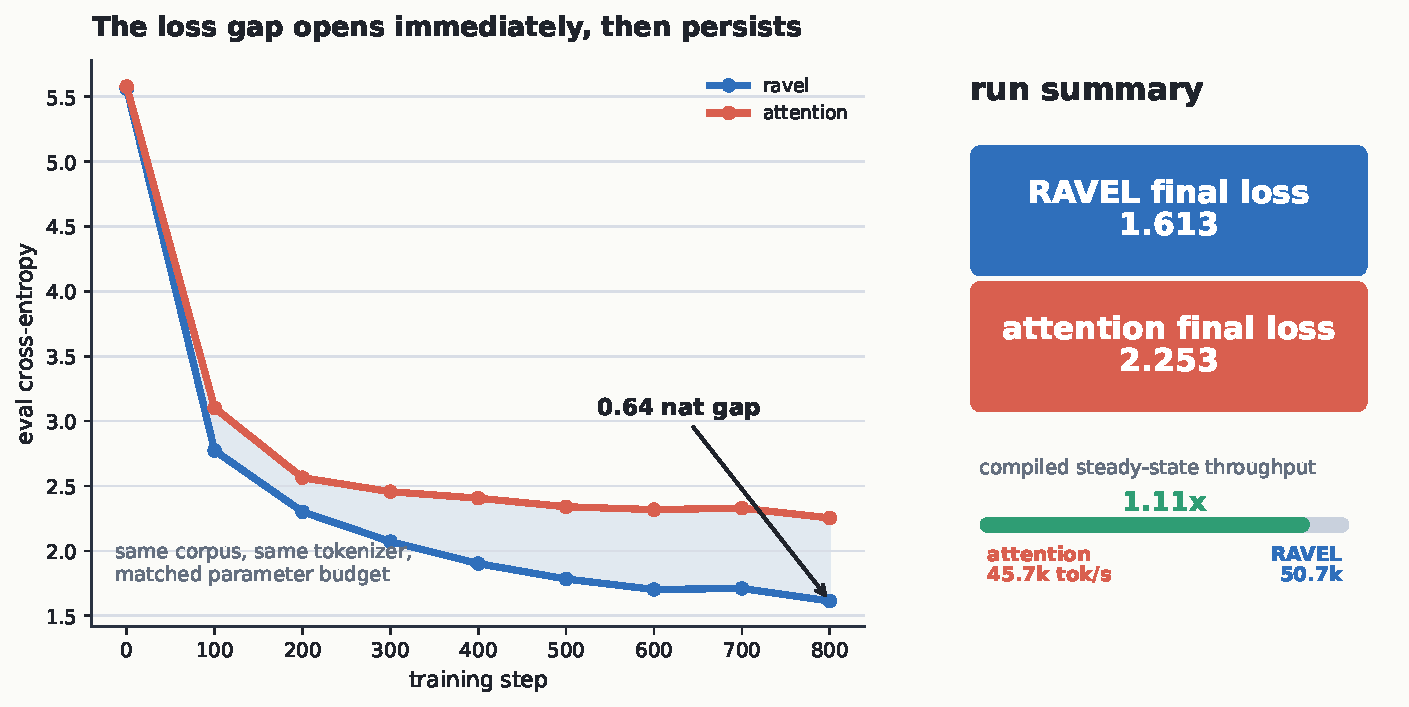
\includegraphics[width=\linewidth]{fig_loss_training.pdf}
  \caption{TinyStories comparison. RAVEL reaches lower evaluation loss than a parameter-matched softmax-attention baseline and is faster in the compiled steady-state training loop for this run.}
  \label{fig:loss}
\end{figure}

\subsection{Where the loss advantage comes from}

The diagnostic slices in Figure~\ref{fig:diagnostics} ask whether the loss gap is consistent with the memory mechanism. At prediction position $j$, RAVEL reads memory using the current input byte and its address variants. The largest current-byte gap occurs when the read key appeared one position earlier: attention-minus-RAVEL NLL is 1.22. The token-class slice shows the largest advantage on punctuation (0.88), with spaces and lowercase bytes also favoring RAVEL. This supports a mechanism-level interpretation: the model is learning reusable continuation and boundary records quickly.

\begin{figure}[H]
  \centering
  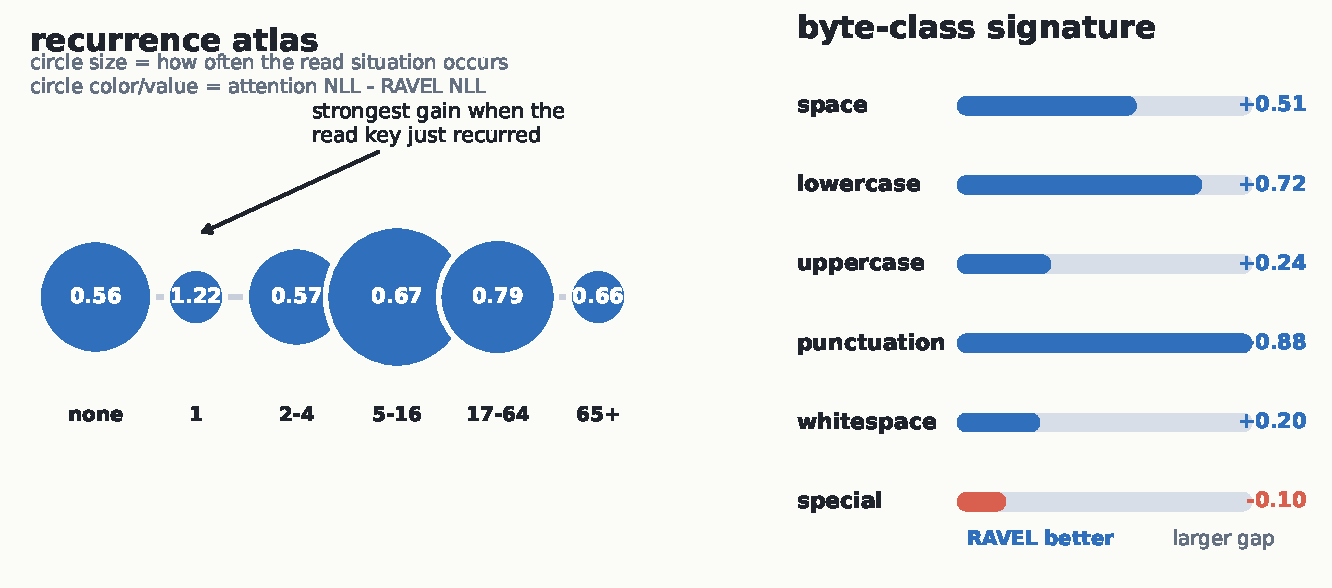
\includegraphics[width=\linewidth]{fig_mechanism_diagnostics.pdf}
  \caption{Mechanism diagnostics. Positive values mean RAVEL assigns lower negative log-likelihood than attention. The advantage is largest when the current read key has just recurred and on boundary-like byte classes such as punctuation and space.}
  \label{fig:diagnostics}
\end{figure}


\subsection{Local learning coefficient / RLCT estimate}

To test whether the loss result is hiding a sharper or more fragile basin, we ran a WBIC-temperature local learning coefficient estimator around both trained checkpoints. The sampler uses fixed training tokens, inverse temperature $\beta=1/\log n$, and the estimator
\[
  \hat{\lambda} = \beta n\left(\mathbb{E}_\beta[L(\theta)] - L^\star\right),
\]
where $L^\star$ is the best loss observed by the local chains. We used $n=2048$ byte-token targets, $\beta=0.131$, three SGLD chains per model, 260 steps per chain, and discarded the first 100 steps as burn-in.

The estimate is 0.203$\pm$0.073 for RAVEL and 0.231$\pm$0.038 for attention (Figure~\ref{fig:rlct}). In this run, RAVEL has lower task loss and a slightly lower local learning coefficient estimate. The result argues against the boring explanation that RAVEL only wins by landing in a sharper local basin.

\begin{figure}[H]
  \centering
  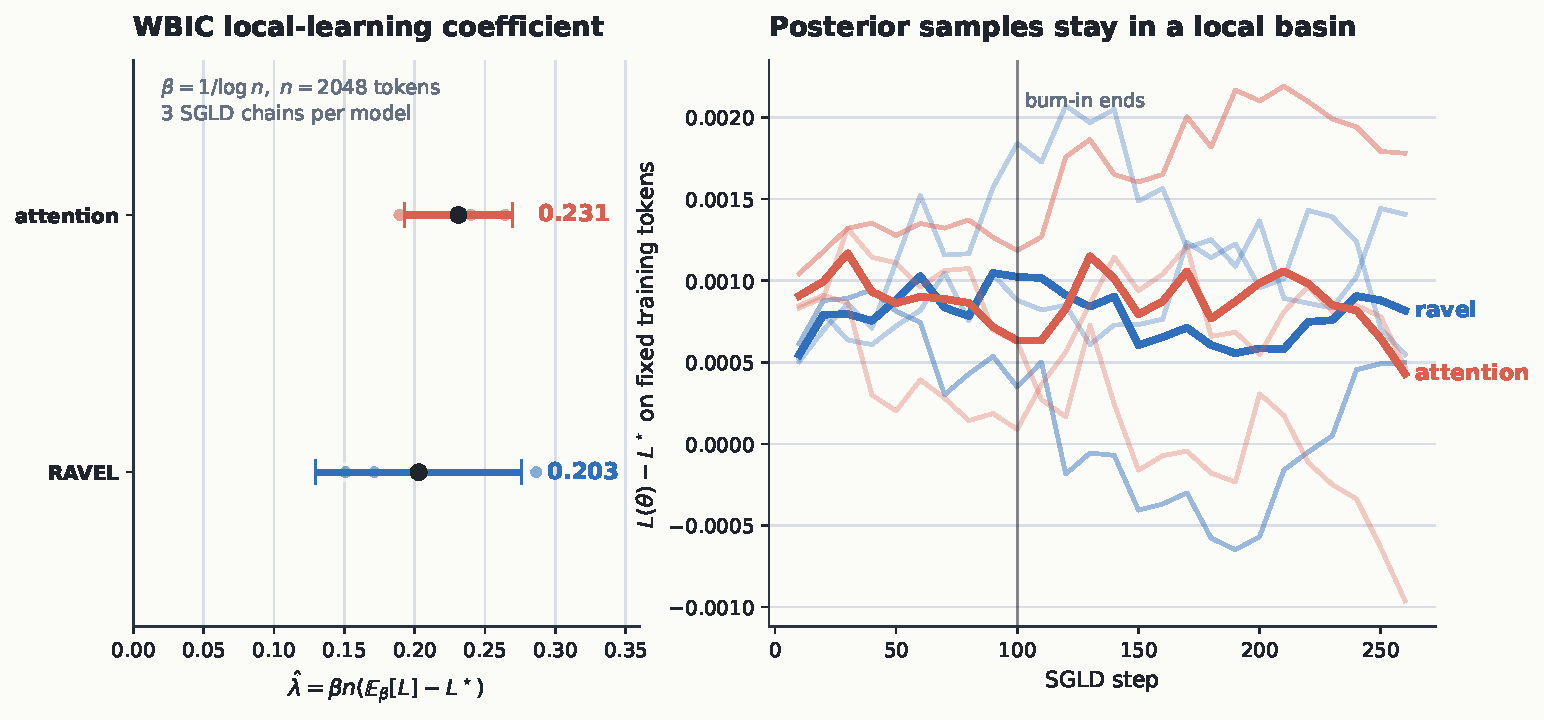
\includegraphics[width=\linewidth]{fig_rlct_probe.pdf}
  \caption{WBIC/local-learning-coefficient estimate around the trained checkpoints. Points show chain estimates; thick intervals show mean $\pm$ chain standard deviation. The right panel shows sampled excess loss after burn-in.}
  \label{fig:rlct}
\end{figure}


\subsection{Speed scaling}

The speed results follow the complexity ledger. At very short contexts, runtime is dominated by constant factors and backend kernel choices. As $T$ grows, attention's quadratic term becomes visible and RAVEL's event lookup stays much flatter. Compiled RAVEL reaches 2.13$\times$ attention throughput at $T=512$ and 3.94$\times$ at $T=1024$ (Figure~\ref{fig:speed-context}).

\begin{figure}[H]
  \centering
  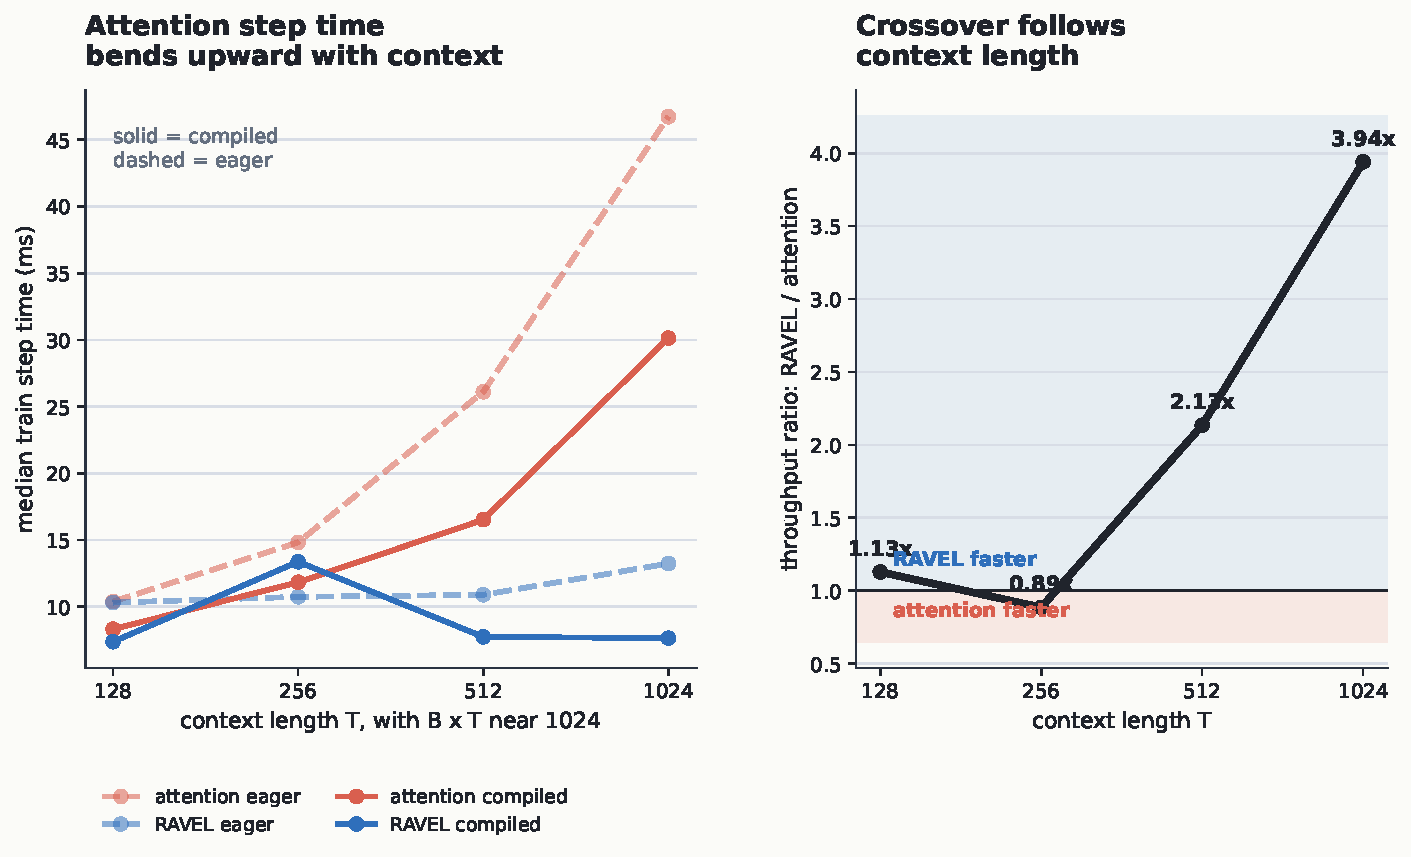
\includegraphics[width=\linewidth]{fig_context_crossover.pdf}
  \caption{Runtime crossover under a constant-token context sweep. The benchmark holds $BT \approx 1024$ and increases $T$. RAVEL is near parity at short contexts but reaches 2.13$\times$ attention throughput at $T=512$ and 3.94$\times$ at $T=1024$ in compiled mode.}
  \label{fig:speed-context}
\end{figure}

The fixed-context sweep checks that this is not merely a batch-size artifact. At $T=512$, the compiled RAVEL advantage grows from 1.74$\times$ at 512 tokens/step to 2.62$\times$ at 2048 tokens/step (Figure~\ref{fig:speed-tokens}).

\begin{figure}[H]
  \centering
  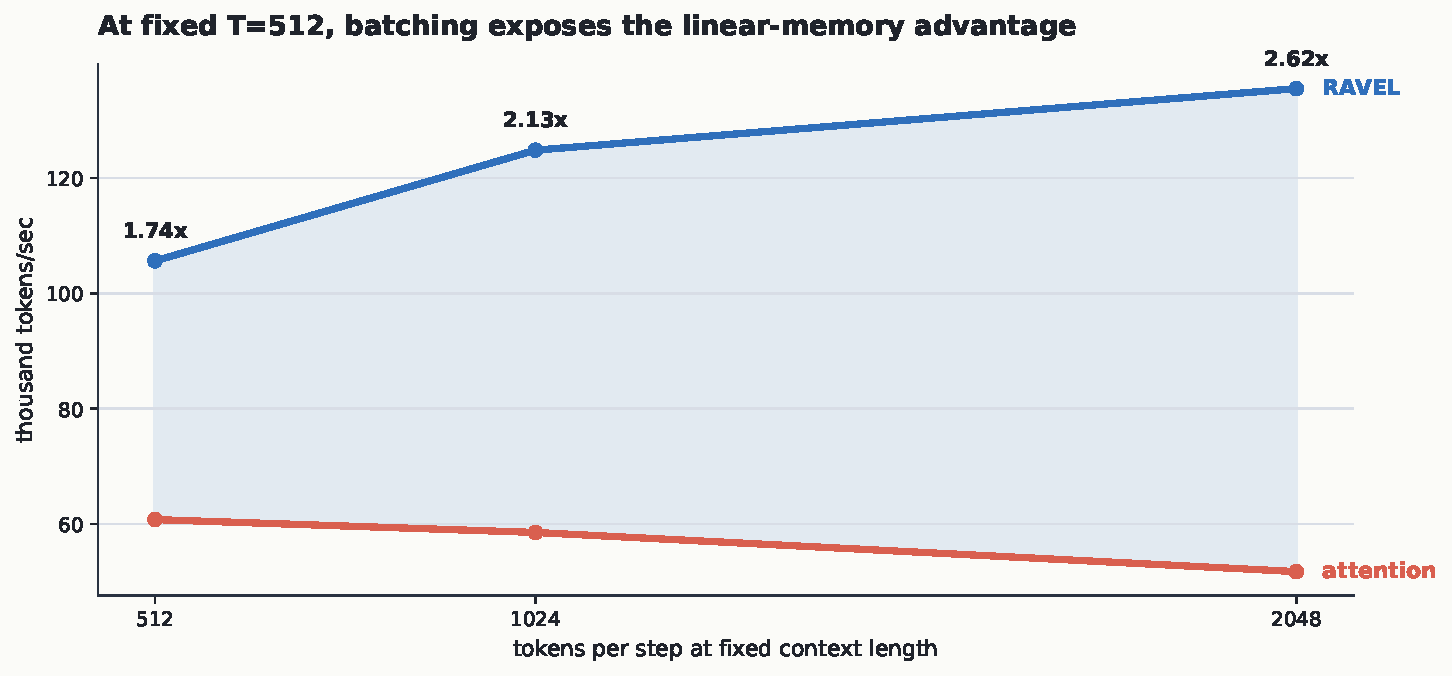
\includegraphics[width=\linewidth]{fig_fixed_t_scaling.pdf}
  \caption{Fixed-context throughput at $T=512$. As more tokens are packed into each training step, RAVEL's advantage grows rather than disappearing.}
  \label{fig:speed-tokens}
\end{figure}

The attention score tensor explains the direction of the crossover. In the context sweep, $BT$ is held near 1024, but the attention score tensor still grows from 6 MiB at $T=128$ to 48 MiB at $T=1024$ per forward pass across layers (Figure~\ref{fig:pressure}). RAVEL does not form this tensor.

\begin{figure}[H]
  \centering
  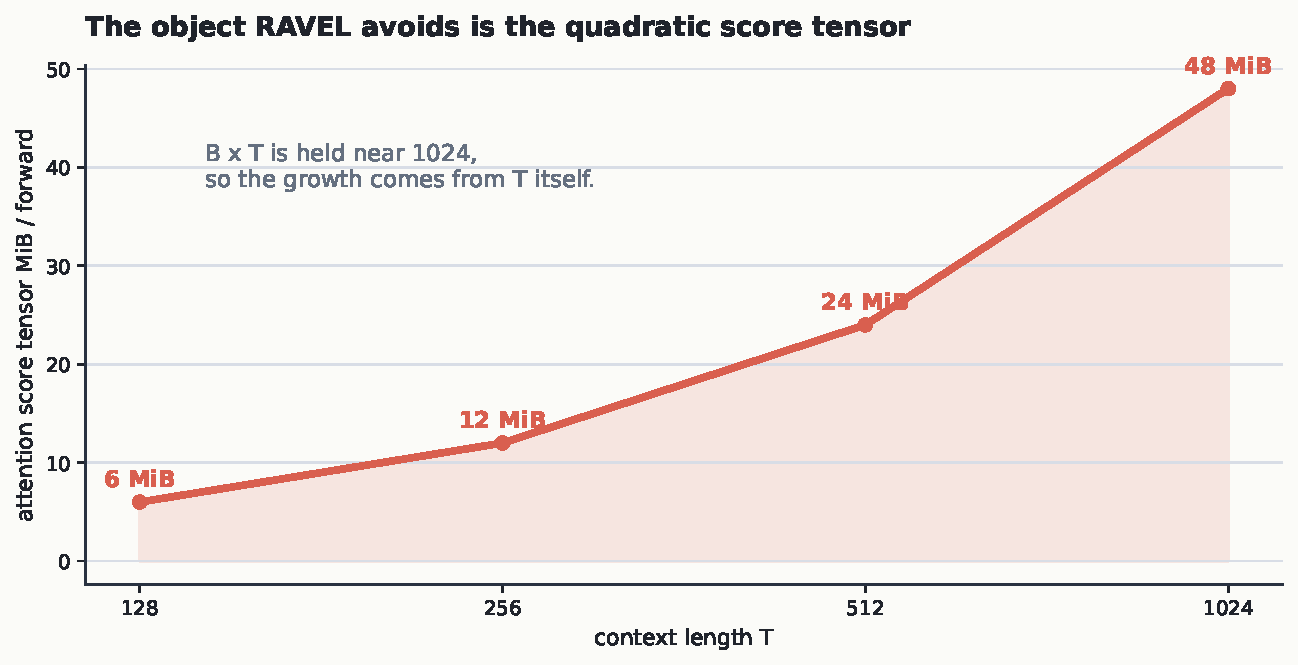
\includegraphics[width=0.86\linewidth]{fig_attention_pressure.pdf}
  \caption{Attention's causal score tensor grows quadratically with context length. In the context sweep, $BT$ is held near 1024, so the growth comes from $T$ itself rather than from processing more tokens per step.}
  \label{fig:pressure}
\end{figure}

\section{Discussion}

The experiments support three claims. First, exact addressed memory trains cleanly on natural byte-level text and beats the parameter-matched attention baseline in this controlled 200k-parameter run. Second, the gain has the mechanism signature RAVEL should have: it concentrates around repeated read keys and boundary-like bytes where exact recurrence is immediately useful. Third, the runtime separates in the direction predicted by the complexity analysis: attention pays for all-pairs scores, while RAVEL pays for event records and fusion.

The next engineering targets are also clear. The current training path uses portable PyTorch sort/search/gather rather than a fused latest-record kernel. The product-code router is hard and frozen; a stronger version should use straight-through routing, differentiable address learning, or explicitly randomized hash families. The present paper establishes the operator, the algorithms, and the first scaling audit. The obvious next version is a fused event-memory kernel plus a trainable router.

\section{Conclusion}

RAVEL-LM replaces dense attention with exact addressed event memory. In byte-level experiments, this gives faster learning and long-context speedups while preserving a clear mechanism: retrieve the latest previous payload with the same address. The central result is algorithmic as much as empirical. Useful recurrence can be implemented as event lookup and fusion, without constructing a quadratic attention matrix.

\end{document}
